\documentclass[12pt]{article}

\usepackage{report}

\usepackage[utf8]{inputenc} % allow utf-8 input
\usepackage[T1]{fontenc}    % use 8-bit T1 fonts
\usepackage[colorlinks=true, linkcolor=black, citecolor=blue, urlcolor=blue]{hyperref}       % hyperlinks
\usepackage{url}            % simple URL typesetting
\usepackage{booktabs}       % professional-quality tables
\usepackage{amsfonts}       % blackboard math symbols
\usepackage{nicefrac}       % compact symbols for 1/2, etc.
\usepackage{microtype}      % microtypography
\usepackage{lipsum}		% Can be removed after putting your text content
\usepackage{graphicx}
\usepackage{natbib}
\usepackage{doi}
\usepackage{float}
% \setcitestyle{aysep={,}}



\title{Using Simultaneous Perturbation Stochastic Approximation to Design a Three-String Network With Strictly Odd-Harmonics}

\author{Srinivas Vadhiraj\\
\AND
Mentor: Saba Goodarzi
\AND
\AND
\AND
\AND
	Institue for Computing in Research\\
\AND
}

% Uncomment to remove the date
\date{August 2023}

% Uncomment to override  the `A preprint' in the header
\renewcommand{\undertitle}{Summer Research}
% \renewcommand{\shorttitle}{}


\begin{document}
\maketitle

\newpage
\tableofcontents
\thispagestyle{empty}

% \newpage
% \thispagestyle{empty}
% \begin{abstract}
% 	\lipsum[1]
% \end{abstract}


% keywords can be removed
% \keywords{First keyword \and Second keyword \and More}


\newpage
\setcounter{page}{1}
\section{Introduction to Acoustics}
\begin{figure}[htbp]
    \centering
    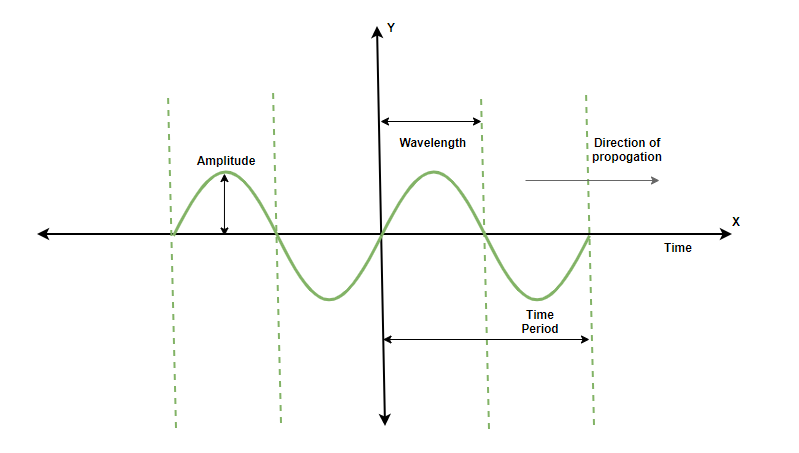
\includegraphics[width=\textwidth,height=.6\textheight,keepaspectratio]{diagram.png}
    \caption{Example of a Simple Waveform (Single Sinusoidal Function)}
    \label{fig:simple_waveform}
\end{figure}

Sound, as an acoustic phenomenon, is fundamentally a propagating waveform, characterized by a pressure disturbance in a medium, typically air. Understanding the visual representation of sound waveforms is crucial in numerous scientific and engineering applications. Sound waveforms can be effectively represented in a pressure vs. time graph, as depicted in Figure \ref{fig:simple_waveform}. Figure \ref{fig:simple_waveform} exemplifies a simple waveform, specifically a single sinusoidal function, which serves as a foundational building block in acoustical analysis.

The analysis of simple waveforms is of significance due to their inherent characteristics, including amplitude and wavelength. However, the most salient property of interest is the frequency of the waveform. When we combine two or more such simple sinusoids together, we obtain a complex waveform. It can be of great use to take some of these complex waveforms and decompose them into their simple sinusoidal components.

\begin{figure}[htbp]
    \centering
    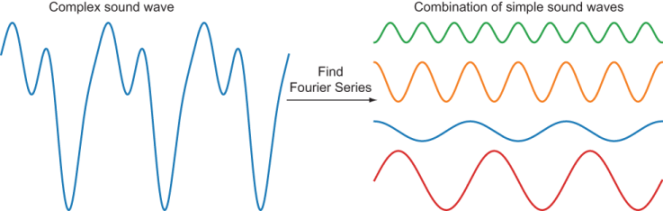
\includegraphics[width=\textwidth,height=.6\textheight,keepaspectratio]{decomposing_wave.png}
    \caption{Decomposing a Periodic Signal Using Fourier Series}
    \label{fig:fourier_series}
\end{figure}

In the field of acoustics, Fourier series emerges as such a tool to conduct such decomposition. Figure \ref{fig:fourier_series} visually demonstrates the process of decomposing a periodic signal using Fourier series, revealing the distinct single-frequency simple sinusoids that constitute the complex waveform. 

\begin{figure}[htbp]
    \centering
    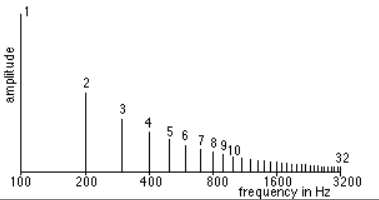
\includegraphics[width=\textwidth,height=.6\textheight,keepaspectratio]{spectrum.png}
    \caption{Amplitudes of Components of a Waveform with Respect to Frequency}
    \label{fig:amplitudes_frequency}
\end{figure}

To delineate the resonance phenomenon further, Figure \ref{fig:amplitudes_frequency} depicts the amplitudes of the individual frequency components with respect to their respective frequencies. Notably, the fundamental frequency, prominently identified at 100 Hz, exhibits the highest amplitude, succeeded by the harmonically related overtones at 200 Hz, 300 Hz, 400 Hz, and so forth. These overtones, or any frequency higher than the fundamental, encompass integer multiples of the fundamental frequency and collectively form a harmonic spectrum of the sound waveform.

In the specific case illustrated in Figure \ref{fig:amplitudes_frequency}, the harmonic spectrum is the set of positive integers from 1 to 32, {1, 2, ..., 32}, a harmonic sequence. Such harmonic spectra are of interest in acoustical studies and provide insights into the vibrational behavior of the system.

In summary, the visual representation of sound waveforms and the application of Fourier series to decompose complex waveforms into their constituent frequency components offer a powerful framework for comprehending acoustical phenomena. The analysis of resonant frequencies and harmonic spectra significantly contributes to the understanding and characterization of diverse acoustic systems, thus paving the way for a an exploration of sound!
\section{Three-String Network with Strictly Odd Harmonics}

\begin{figure}[htbp]
    \centering
    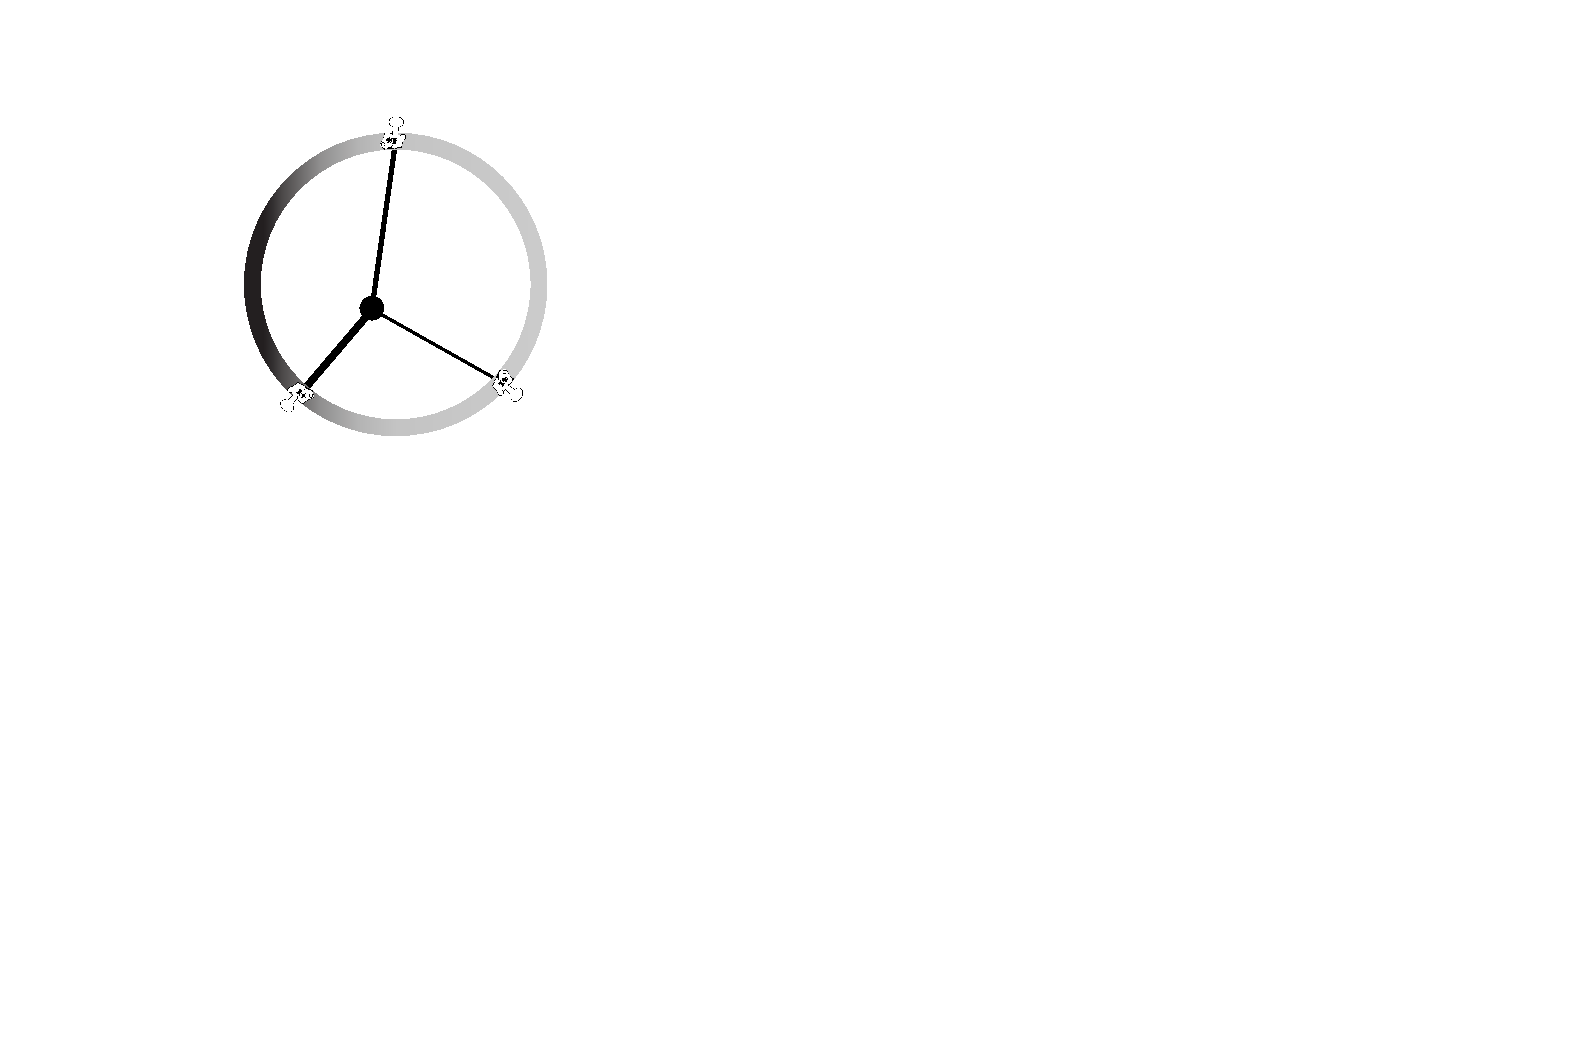
\includegraphics[width=0.5\textwidth]{HoopArtistsConception.pdf}
    \caption{Three-String Network}
    \label{fig:three_string_network}
\end{figure}

The primary objective of this research was to create a three-string network (Figure \ref{fig:three_string_network}) that produces a spectrum consisting of strictly odd harmonics. In a three-string network, we can change each of the three strings' lengths, mass densities, tensions, and the center mass, resulting in a total of ten parameters. To find the resonant frequencies of a three-string design, we find the roots of the following spectral equation:

\[s(\lambda) \equiv \sum_{j=1}^3\sqrt{\tau_j\mu_j} \cos\left(\frac{l_j\sqrt{\mu_j}}{\sqrt{\tau_j}}\lambda\right)\prod_{\substack{k\neq j \\ k=1}}^3 \sin\left(\frac{l_k\sqrt{\mu_k}}{\sqrt{\tau_k}}\lambda\right) + M\lambda \prod_{j=1}^3\sin\left(\frac{l_j\sqrt{\mu_j}}{\sqrt{\tau_j}}\lambda\right)\]

\begin{figure}[htbp]
    \centering
    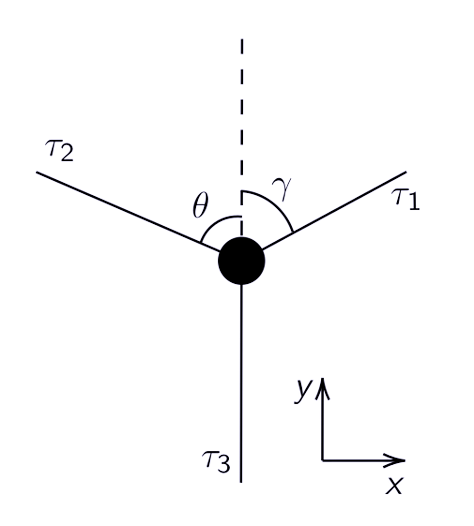
\includegraphics[width=0.5\textwidth]{theta_gamma.png}
    \caption{Newton's Second Law for Tensions}
    \label{fig:newtons_second_law}
\end{figure}

To ensure the physical feasibility of the string configuration, we refer to Newton's second law (Figure \ref{fig:newtons_second_law}), which gives the following equations:

\textbf{Newton's second law in the $x$-direction:}
\[\tau_1\sin\gamma = \tau_2\sin\theta\]

\textbf{Newton's second law in the $y$-direction:}
\[\tau_3 = \tau_2\cos \theta + \tau_1\cos\gamma\]

Using this, we can derive the following ratios for the tensions:

\[\frac{\tau_1}{\tau_3} = \frac{\sin(\theta)}{\sin(\gamma+\theta)}\]

\[\frac{\tau_2}{\tau_3} = \frac{\sin(\gamma)}{\sin(\gamma+\theta)}\]

\begin{figure}[H]
\centering
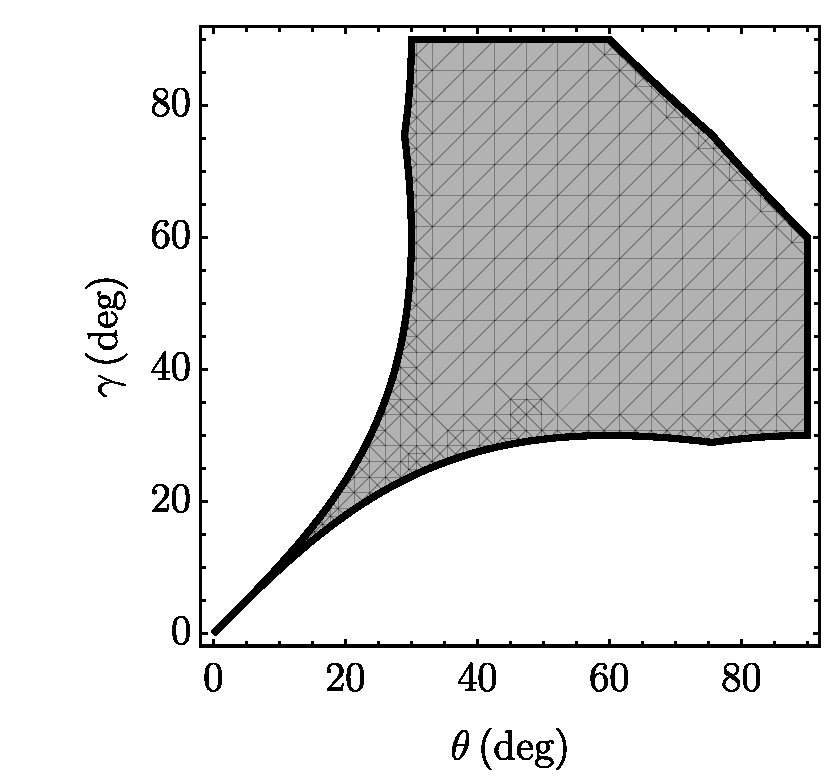
\includegraphics[width=0.5\textwidth]{anglediagram1.pdf}
\caption{Feasible Values of $\theta$ and $\gamma$.}
\label{fig:theta_gamma}
\end{figure}

The values of theta and gamma that satisfy these equations are depicted in Figure \ref{fig:theta_gamma}, where the shaded region represents valid pairs of $\theta$ and $\gamma$.

\begin{figure}[H]
\centering
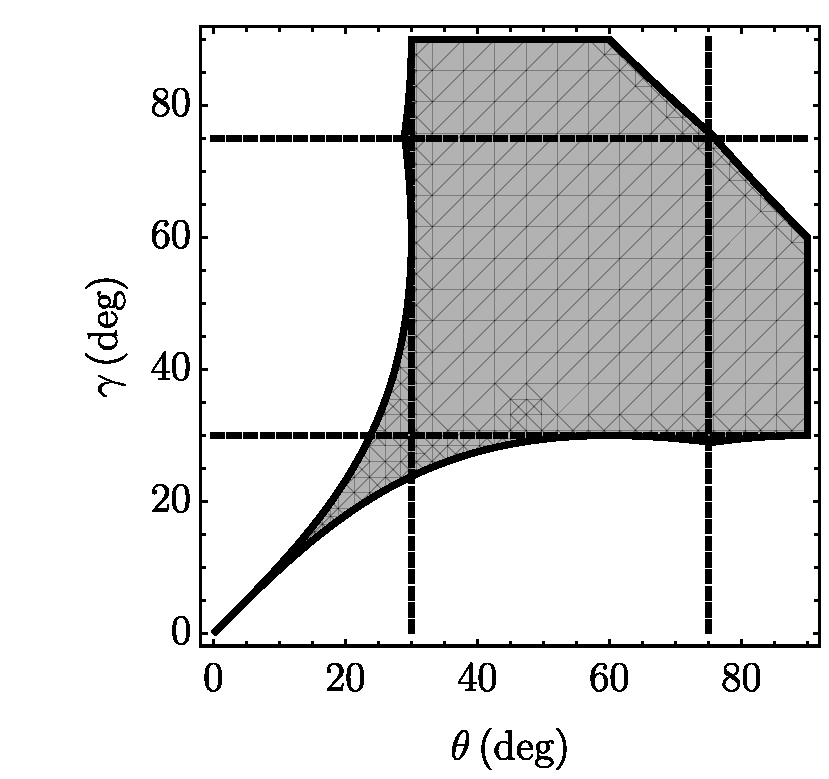
\includegraphics[width=0.5\textwidth]{anglediagram2.pdf}
\caption{Middle Section Partition}
\label{fig:middle_section_partition}
\end{figure}

To further restrict the analysis, we focus on the middle section partition as seen in Figure \ref{fig:middle_section_partition}. Thus, we set bounds on theta and gamma to be between 30 and 75 degrees, and the others as follows:
\[\theta, \gamma \in [30, 75] \text{\textdegree}\]
\[l_1, l_2, l_3 \in [1, 100] \text{(m)}\]
\[\mu_1, \mu_2, \mu_3 \in [0.001, 1] (\frac{\text{kg}}{\text{m}})\]
\[\text{Center Mass} \in [0, 1] \text{(kg)}\]

Now that we have established the bounds, we can proceed with the optimization algorithm.

\section{SPSA and Optimization}

In this section, we present the methodology employed for the optimization of the multi-parameterized design problem. Our focus centers on the implementation of the Simultaneous Perturbation Stochastic Approximation (SPSA) algorithm as the hill climbing technique. SPSA offers an efficient way to traverse high-dimensional parameter space, consisting of $\theta$, $\gamma$, three lengths ($l_1, l_2, l_3$), three $\mu$ values ($\mu_1, \mu_2, \mu_3$), and the center mass, enabling us to find the global optimum of such a function.

\subsection{SPSA: Simultaneous Perturbation Stochastic Approximation}

SPSA is as a powerful optimization algorithm, adept at navigating multi-dimensional search spaces and is particularly well-suited for problems involving noisy and non-differentiable objective functions, making it highly applicable to engineering and scientific disciplines where exact derivatives are often impractical or unavailable.

The underlying principle of SPSA is to stochastically perturbate during each iteration through the addition and subtraction of stochastically generated deltas to the parameter values. By evaluating the objective function at two perturbed points simultaneously, SPSA efficiently estimates the gradient, resulting in  convergence with respect to the number of function evaluations. As a result, SPSA requires only a smaller number of evaluations compared to other gradient-based optimization methods, making it useful for computationally expensive optimization tasks.

\subsection{Modifying SPSA for the Task at Hand}

While SPSA offers great promise, applying it directly to the 9-dimensional parameter space may lead to limitations in terms of convergence speed and solution quality. To overcome this, a strategic modification is proposed to enhance the algorithm's performance for the specific design task.

The central idea revolves around the utilization of a bitmask approach to guide the selection of parameters for addition or subtraction during each iteration. The bitmask serves as a binary representation, with each bit corresponding to a parameter, indicating whether to add the respective delta or not. This enables us to perform targeted updates to specific subsets of variables at any given time.

The iterative process involves cycling through all possible masks, generating diverse spectra of designs for each configuration. This approach has the advantage of diversifying the exploration of the parameter space, significantly increasing the probability of converging quicker, be it to a local or global optimum.

While this modified approach increases the computational burden, demanding 256 times more operations than traditional SPSA, its potential to converge to the roots more rapidly justifies the additional complexity. 

\section{Results}

This section presents results from running both versions of SPSA, two directional and bitmask, and aims to compare the rate of convergence toward an optimal solution of both of them. Each pair of images represents the corrpesonding number of iterations in bitmask vs. two directional.

\begin{figure}[htbp]
\centering
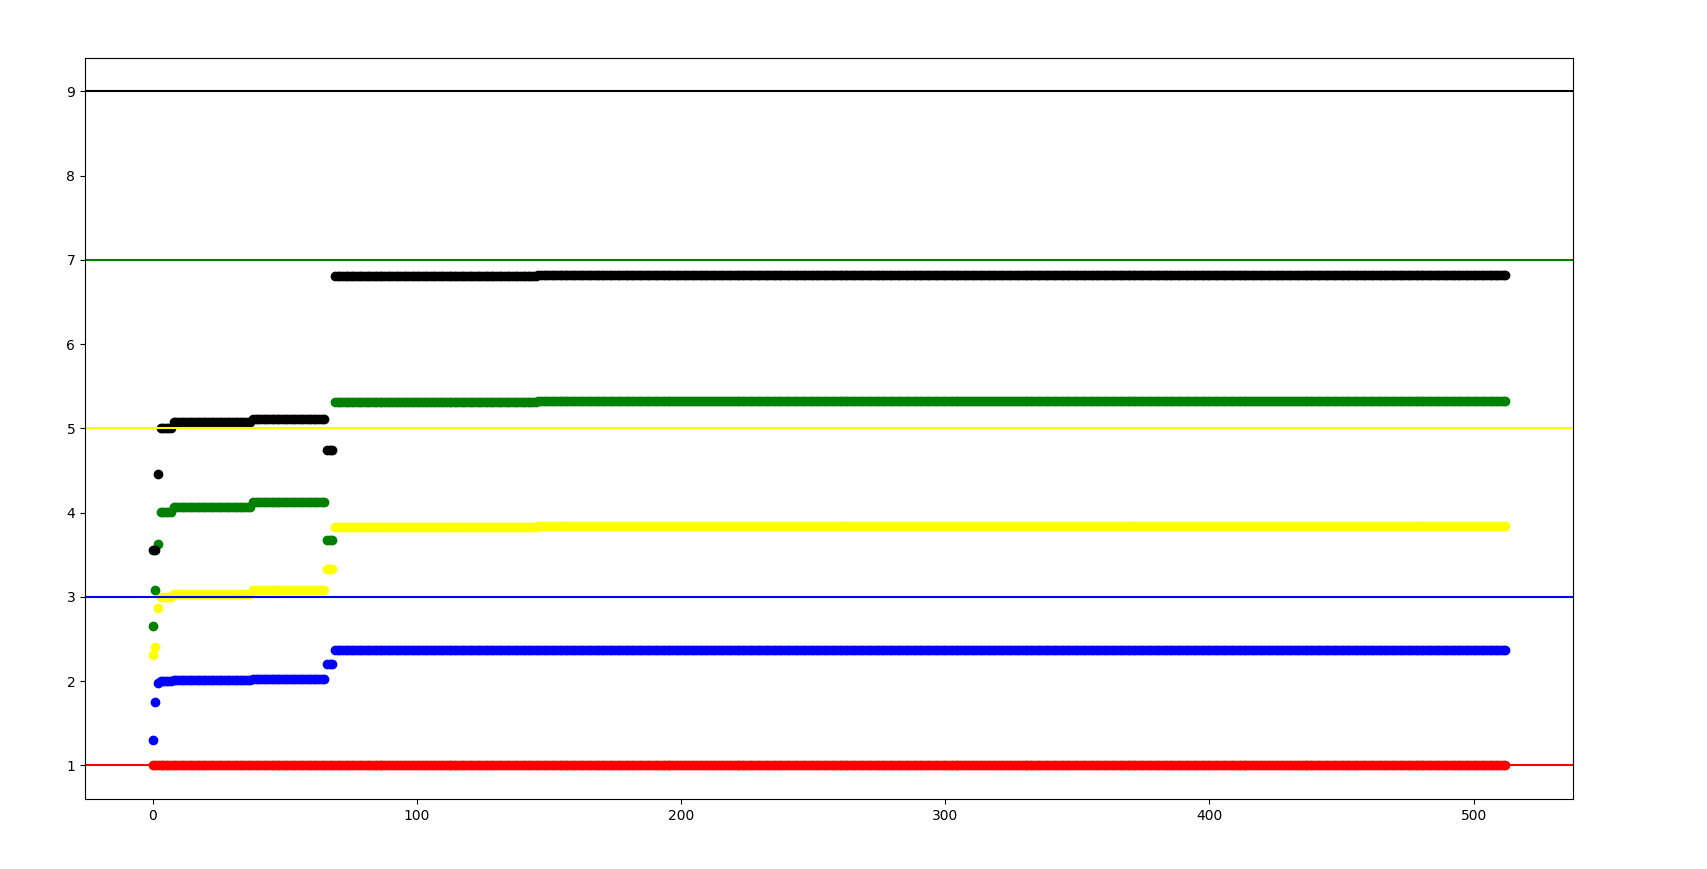
\includegraphics[width=0.6\textwidth]{Two_512.png}
\caption{Two Directional -> 512 Iterations}
\label{fig:result_1}
\end{figure}

\begin{figure}[htbp]
\centering
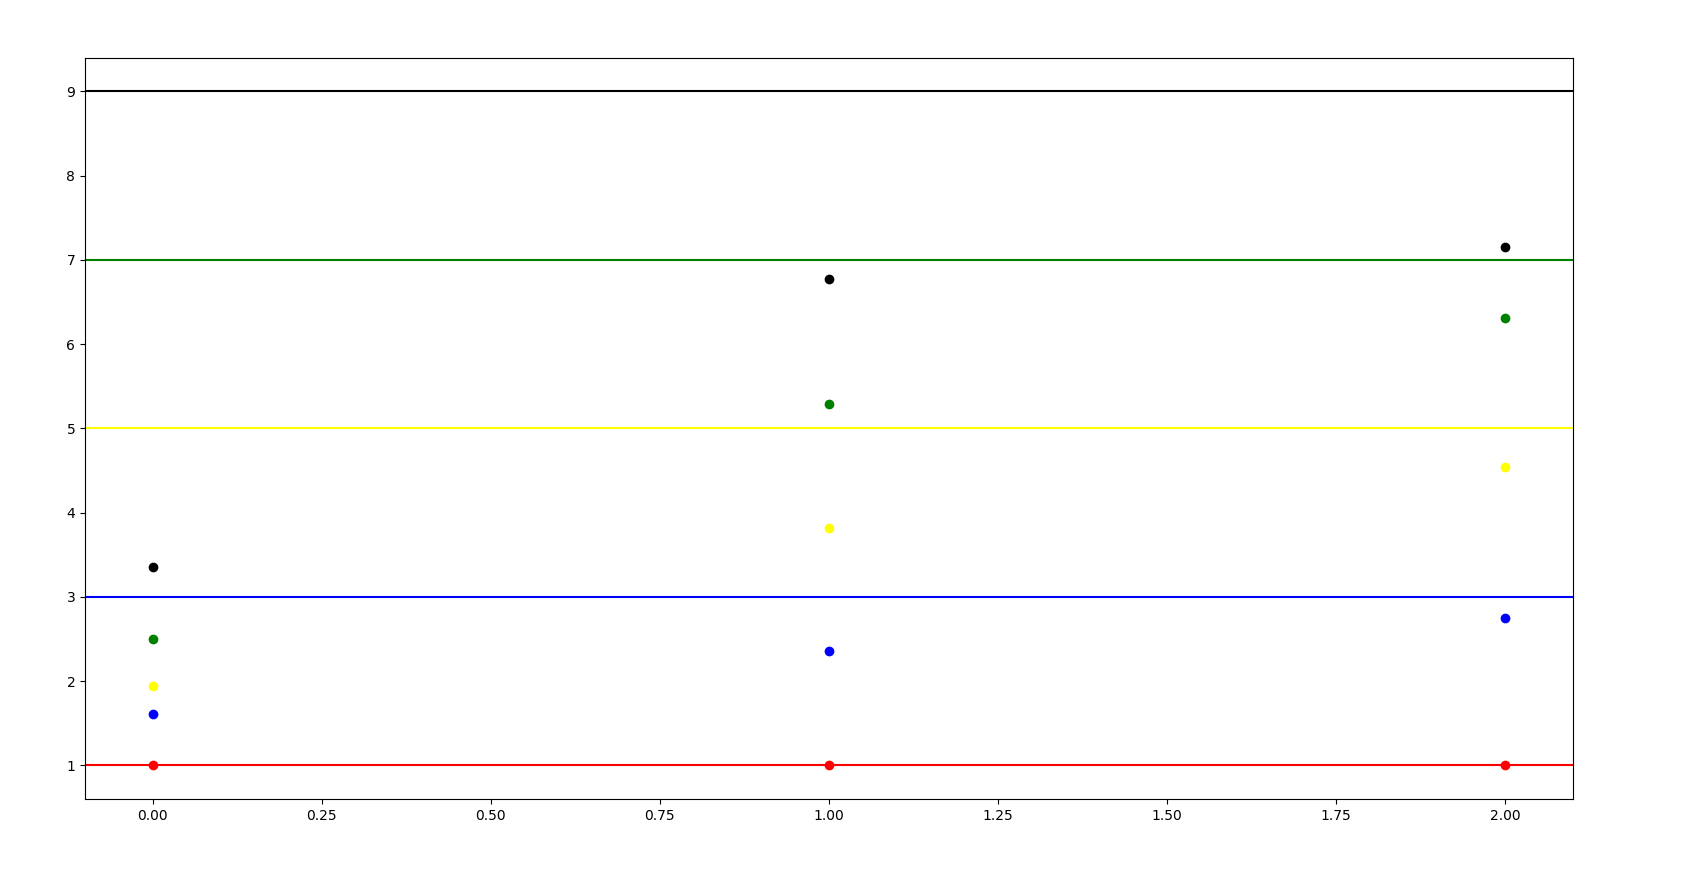
\includegraphics[width=0.6\textwidth]{Bitmask_2.png}
\caption{Bitmask -> 2 Iterations}
\label{fig:result_2}
\end{figure}
\begin{figure}[htbp]
\centering
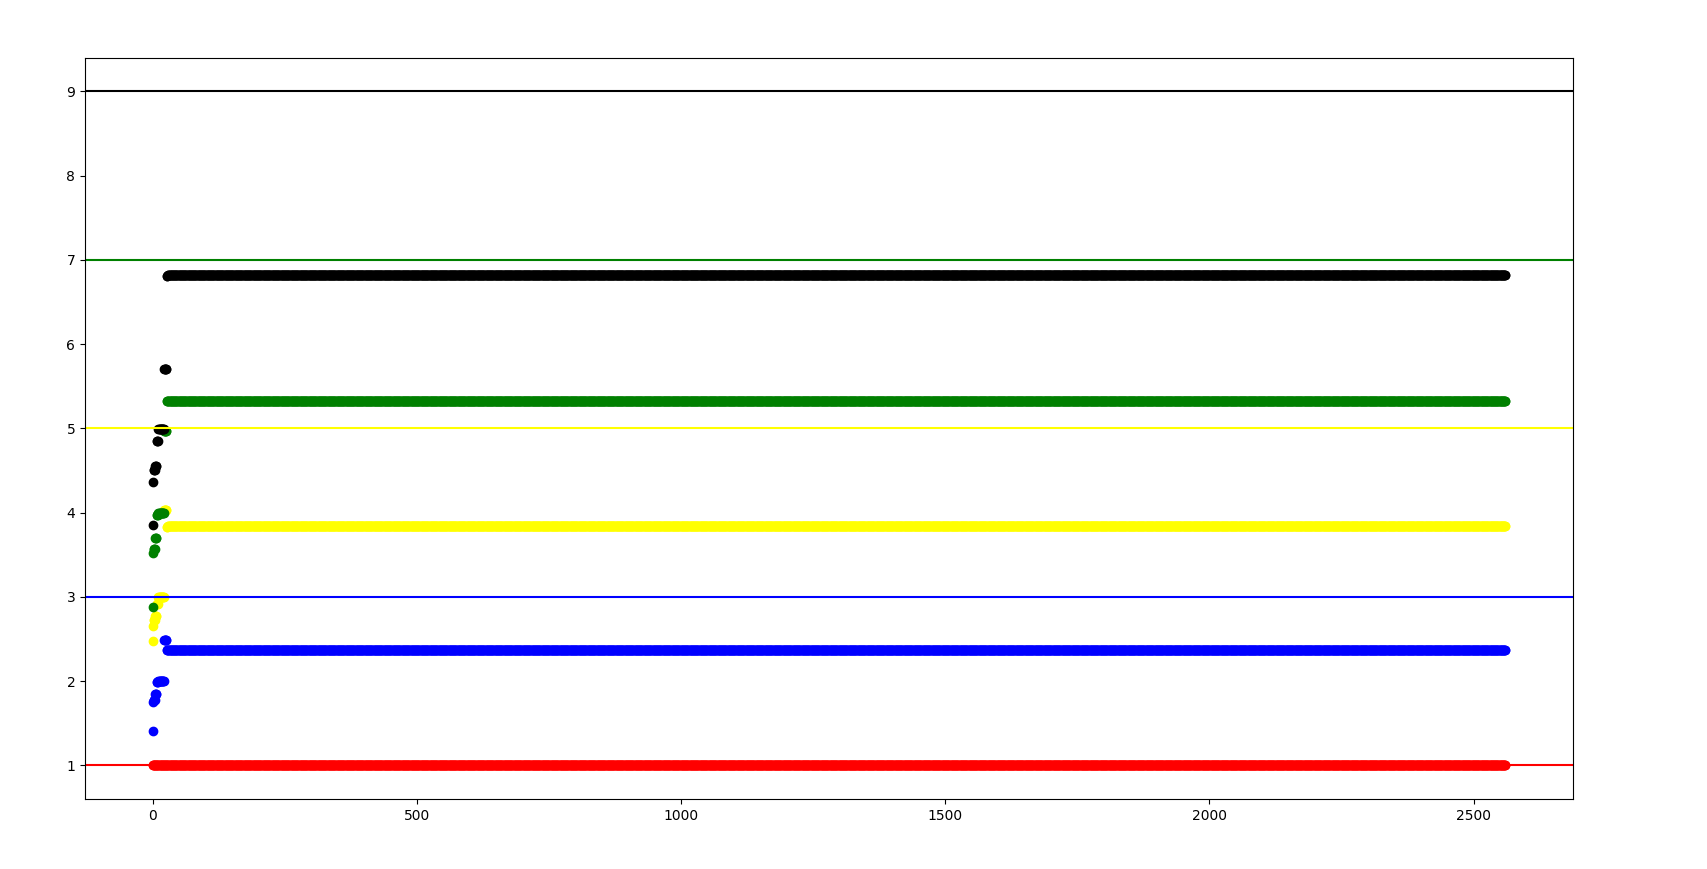
\includegraphics[width=0.6\textwidth]{Two_2560.png}
\caption{Two Directional -> 2560 Iterations}
\label{fig:result_3}
\end{figure}

\begin{figure}[htbp]
\centering
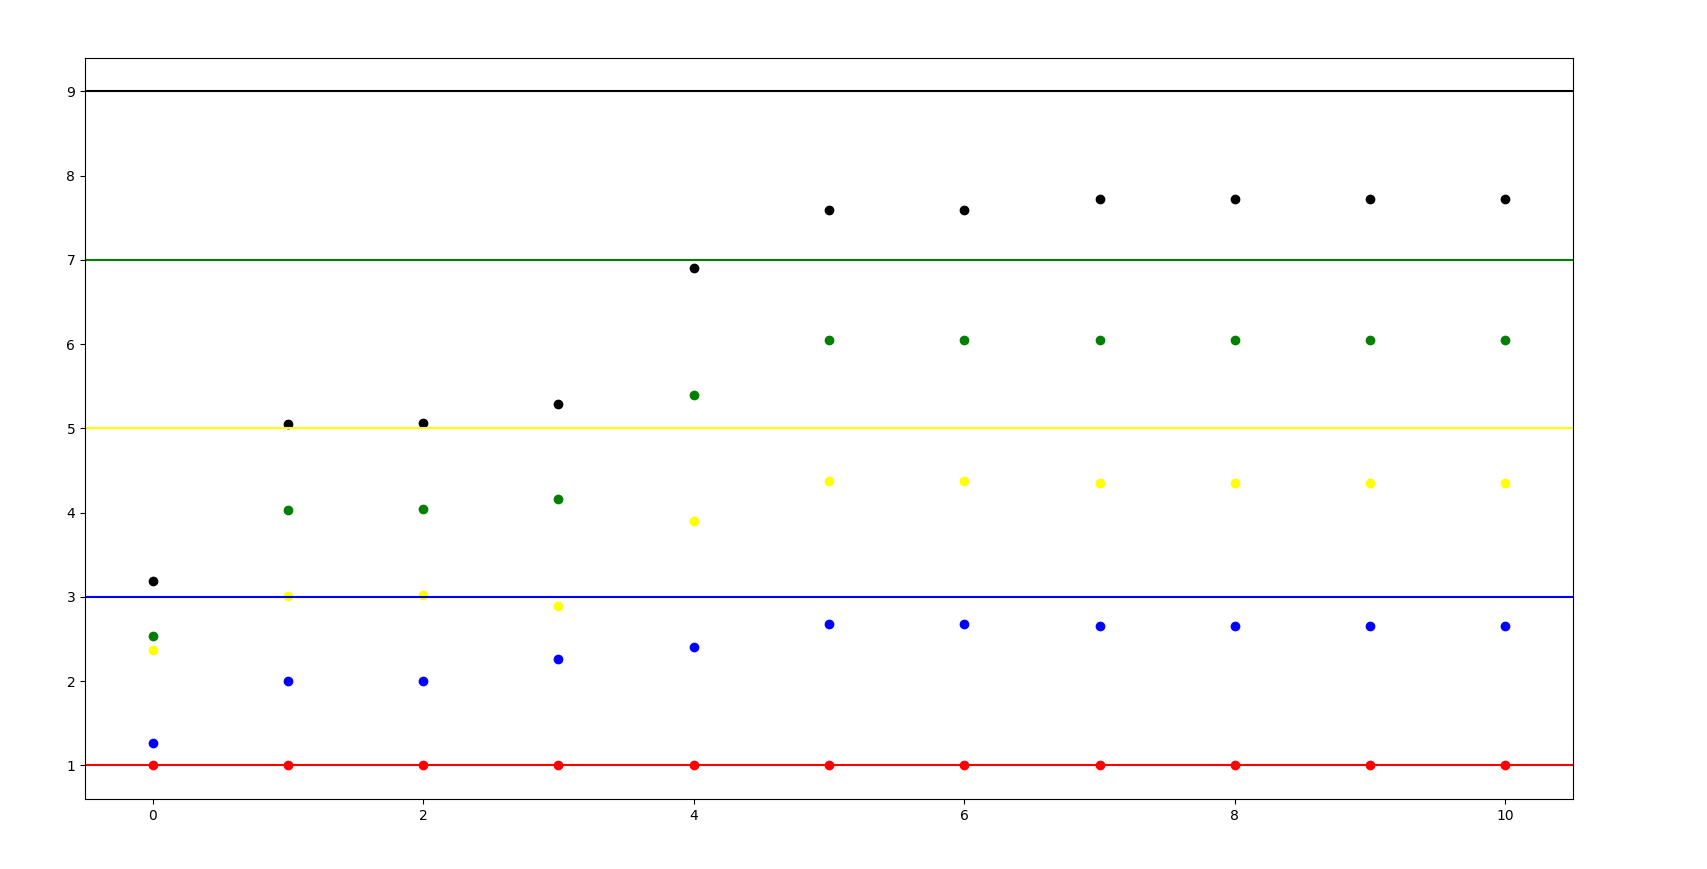
\includegraphics[width=0.6\textwidth]{Bitmask_10.png}
\caption{Bitmask -> 10 Iterations}
\label{fig:result_4}
\end{figure}
\begin{figure}[htbp]
\centering
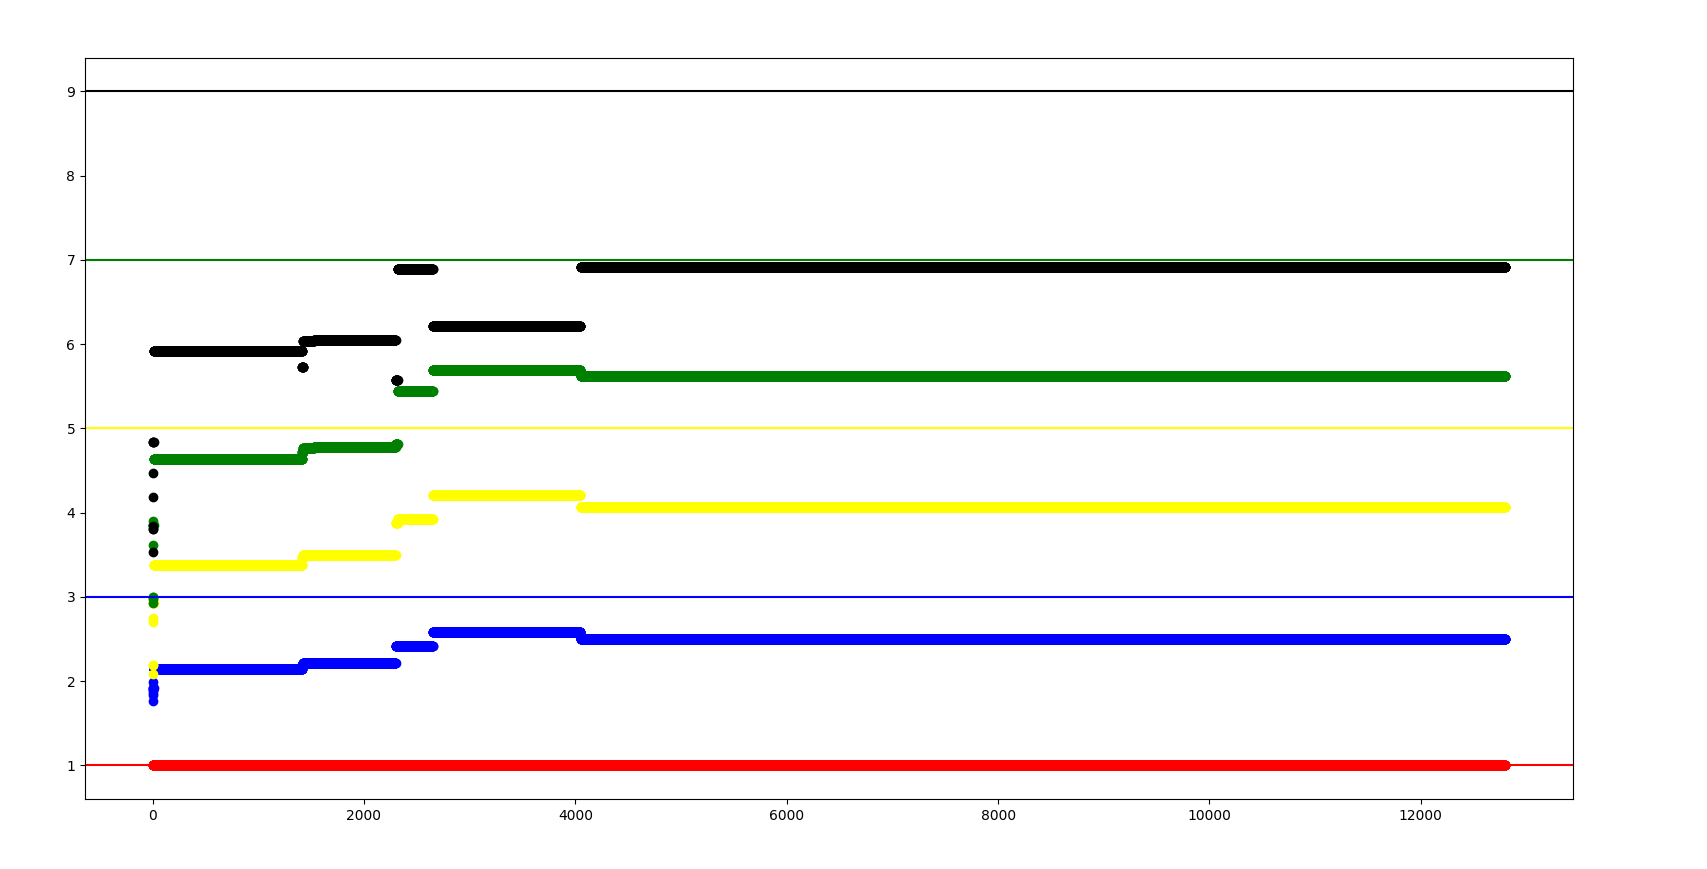
\includegraphics[width=0.6\textwidth]{Two_12800.png}
\caption{Two Directional -> 12800 Iterations}
\label{fig:result_5}
\end{figure}

\begin{figure}[htbp]
\centering
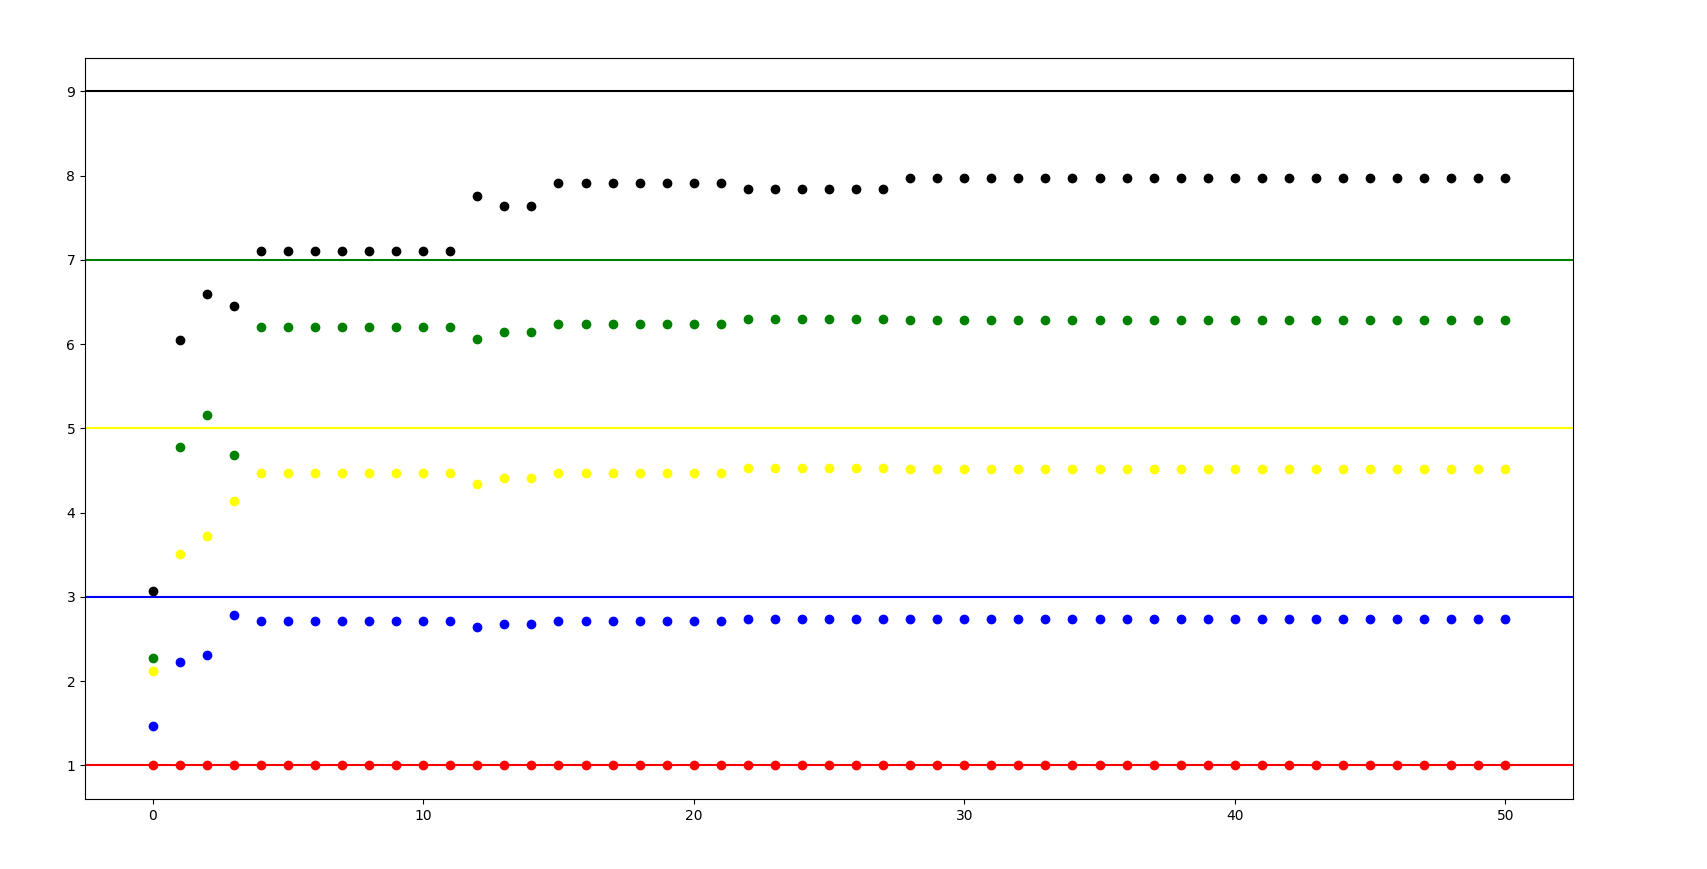
\includegraphics[width=0.6\textwidth]{Bitmask_50.png}
\caption{Bitmask -> 50 Iterations}
\label{fig:result_6}
\end{figure}
\begin{figure}[htbp]
\centering
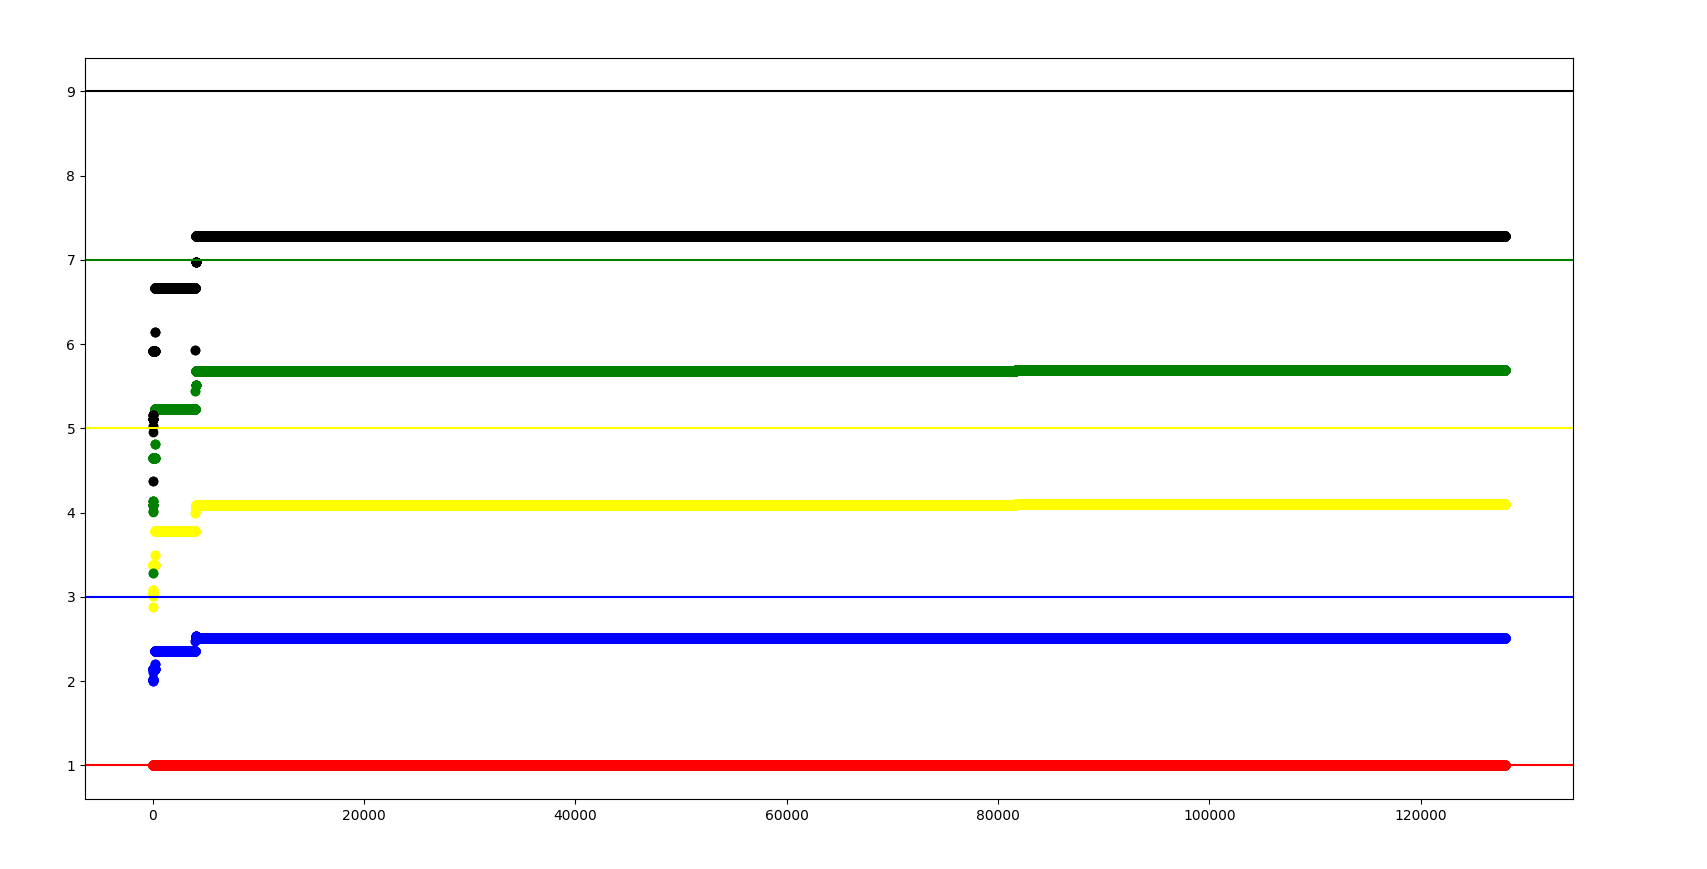
\includegraphics[width=0.6\textwidth]{Two_128000.png}
\caption{Two Directional -> 128000 Iterations}
\label{fig:result_7}
\end{figure}

\begin{figure}[htbp]
\centering
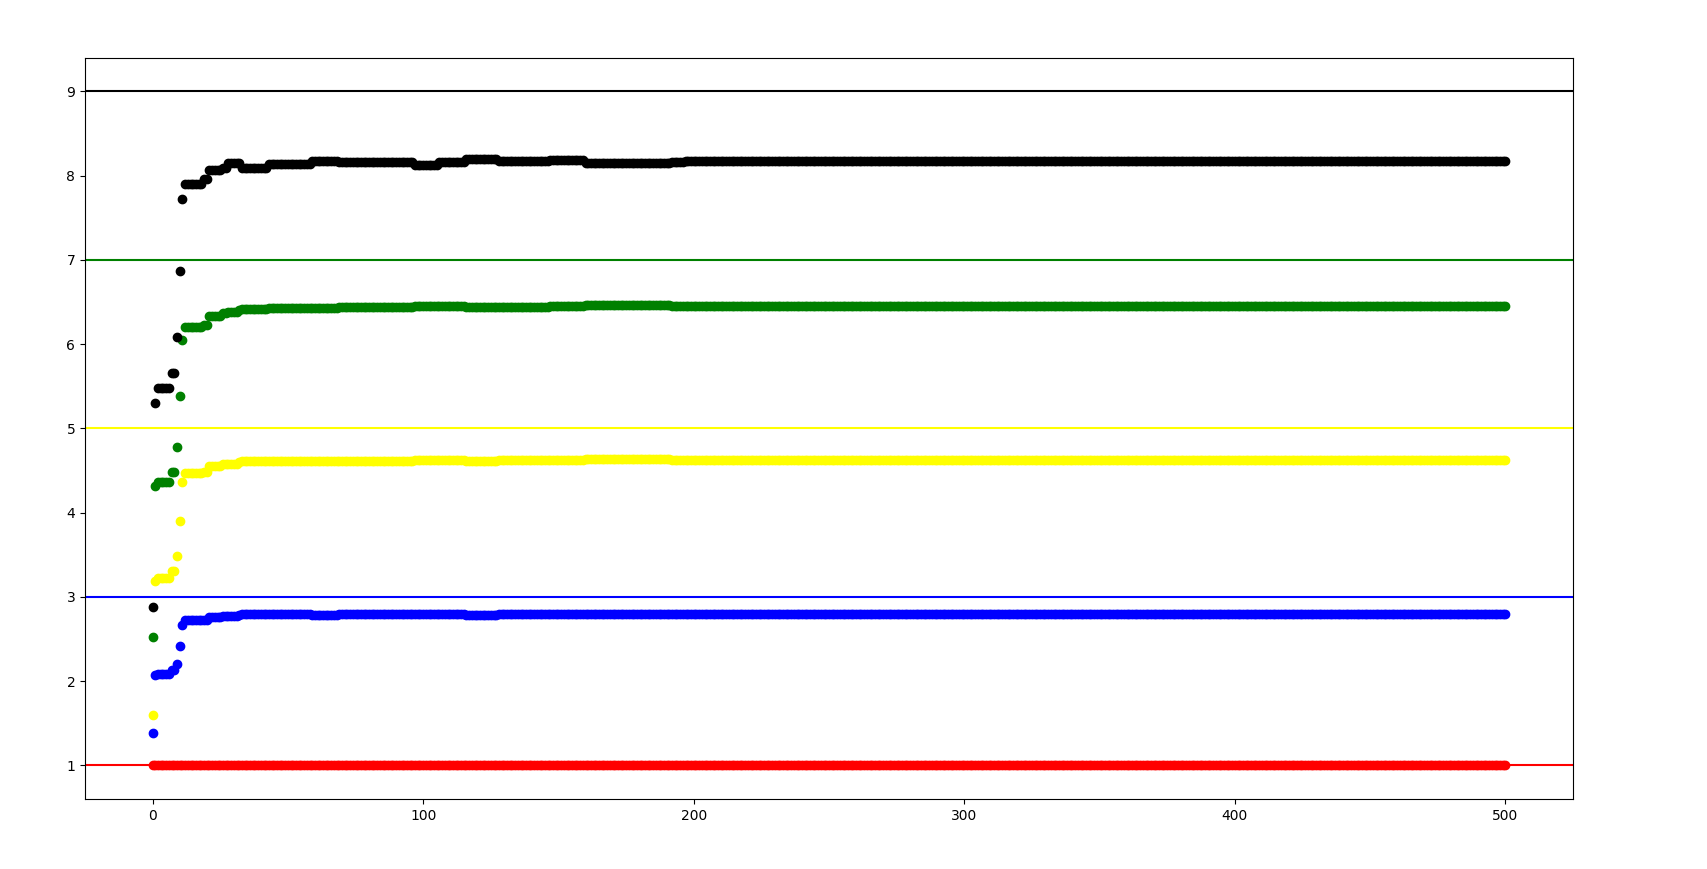
\includegraphics[width=0.6\textwidth]{Bitmask_500.png}
\caption{Bitmask -> 500 Iterations}
\label{fig:result_8}
\end{figure}

\begin{figure}[htbp]
\centering
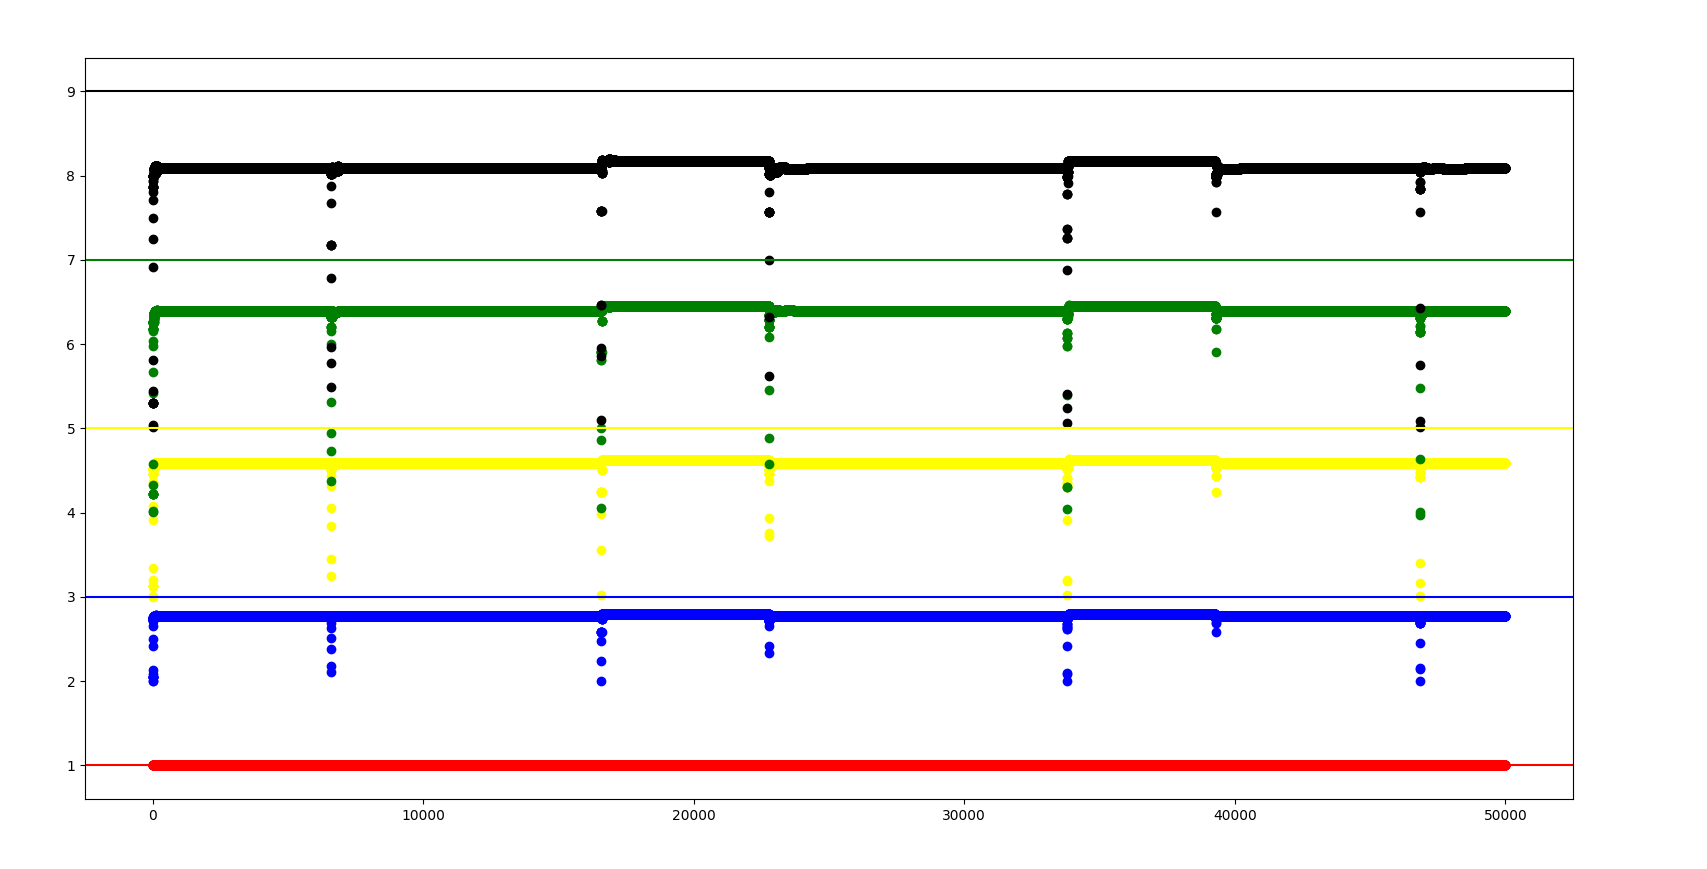
\includegraphics[width=0.6\textwidth]{Bitmask_50000.png}
\caption{Bitmask -> 50000 Iterations}
\label{fig:result_9}
\end{figure}


\subsection{Discussion}

Upon analyzing the results presented in Figures \ref{fig:result_1} to \ref{fig:result_9}, it becomes evident that the achieved roots do not converge as closely as desired. This discrepancy can be attributed to various factors in our optimization process.

Firstly, the limited exploration of the parameter space, focusing only on a subset of the bounds for $\theta$ and $\gamma$, may result in overlooking potential optimal solutions lying outside the specified region. Broadening the exploration bounds for these angles could lead to the discovery of a more desirable design.

Furthermore, it is plausible that we have not run enough iterations or need to increase the failsafe number due to limited computional time, power, and storage.

Additionally, it is feasible that no such three string network exists such that the spectrum is the set of odd numbers! To address this, an avenue for improvement involves generalizing the approach to accommodate $n$-string designs, thereby broadening the search space and potentially uncovering more suitable designs.

To further enhance the optimization process, exploring alternative algorithms such as simulated annealing or genetic algorithms could offer additional insights and potentially overcome the limitations encountered with the current methodology.

\subsection{Further Research}

The investigation into optimizing the design of the multi-string configuration proves to be a compelling avenue for future research. Beyond the immediate modifications discussed, several intriguing possibilities exist to expand and enhance the present study.

In conclusion, this research offers insights into the optimization of multi-string designs, and the findings show different avenues of further exploration to improve the performance and applicability of the designed systems.

% Acknowledgments and References can be added if necessary.


% \bibliographystyle{acl_natbib}
% \bibliography{references}  %%% Uncomment this line and comment out the ``thebibliography'' section below to use the external .bib file (using bibtex) .


%%% Uncomment this section and comment out the \bibliography{references} line above to use inline references.
% \begin{thebibliography}{1}

% 	\bibitem{kour2014real}
% 	George Kour and Raid Saabne.
% 	\newblock Real-time segmentation of on-line handwritten arabic script.
% 	\newblock In {\em Frontiers in Handwriting Recognition (ICFHR), 2014 14th
% 			International Conference on}, pages 417--422. IEEE, 2014.

% 	\bibitem{kour2014fast}
% 	George Kour and Raid Saabne.
% 	\newblock Fast classification of handwritten on-line arabic characters.
% 	\newblock In {\em Soft Computing and Pattern Recognition (SoCPaR), 2014 6th
% 			International Conference of}, pages 312--318. IEEE, 2014.

% 	\bibitem{hadash2018estimate}
% 	Guy Hadash, Einat Kermany, Boaz Carmeli, Ofer Lavi, George Kour, and Alon
% 	Jacovi.
% 	\newblock Estimate and replace: A novel approach to integrating deep neural
% 	networks with existing applications.
% 	\newblock {\em arXiv preprint arXiv:1804.09028}, 2018.

% \end{thebibliography}


\end{document}
